\documentclass[11pt,a4paper]{article}
\usepackage{../shared/hanzocover}
\usepackage[utf8]{inputenc}
\usepackage[T1]{fontenc}
\usepackage{amsmath,amssymb}
\usepackage{graphicx}
\usepackage{booktabs}
\usepackage{hyperref}
\usepackage{xcolor}
\usepackage{listings}
\input{../shared/lstlang}
\usepackage{tikz}
\usetikzlibrary{shapes,arrows,positioning}

\lstset{
    basicstyle=\ttfamily\small,
    keywordstyle=\color{blue},
    commentstyle=\color{gray},
    stringstyle=\color{red},
    breaklines=true,
    frame=single,
    numbers=left,
    numberstyle=\tiny\color{gray}
}

\title{Hanzo Observability Stack: Search, Telemetry,\\and Session Analytics for Production Systems}
\author{Antje Worring, Zach Kelling\thanks{zach@hanzo.ai} \\ \textit{CTO, Hanzo Industries (Techstars '17)}}
\date{2018}

\begin{document}

\hanzocoverpage

\begin{abstract}
We present the Hanzo observability stack, comprising four components developed between 2016 and 2018: a full-text search engine (\texttt{hanzo/search}, April 2018, 16{,}000 commits), a telemetry and metrics pipeline (\texttt{hanzo/telemetry}, June 2018, 8{,}200 commits), a session recording system (\texttt{hanzo/rrweb}, September 2018, 1{,}600 commits), and an event analytics platform for funnel analysis and user behavior tracking. An OpenAPI specification layer (2016) provides contract-first API documentation across all components. This infrastructure became the foundation for Hanzo Insights, the privacy-first analytics platform.
\end{abstract}

\section{Introduction}

Observability in production systems requires three pillars: logs, metrics, and traces. For user-facing applications, a fourth pillar is equally important: behavioral analytics---understanding how users interact with the product. The Hanzo observability stack addresses all four requirements with a unified data pipeline.

The stack was developed incrementally:
\begin{enumerate}
    \item \textbf{OpenAPI specification} (2016): Contract-first API documentation and code generation.
    \item \textbf{Search engine} (April 2018): Full-text indexing of logs, documents, and product catalogs.
    \item \textbf{Telemetry pipeline} (June 2018): Metrics collection, aggregation, and alerting.
    \item \textbf{Session recording} (September 2018): DOM-level replay of user sessions.
\end{enumerate}

Together, these components provide the observability layer for all Hanzo services.

\section{Full-Text Search}

\subsection{Architecture}

The Hanzo search engine (\texttt{hanzo/search}, 16{,}000 commits) provides full-text search, faceted filtering, and relevance ranking across structured and unstructured data. It indexes commerce data (products, orders, customers), application logs, and documentation.

\subsection{Indexing Pipeline}

Documents enter the search engine through a write-ahead log:

\begin{enumerate}
    \item \textbf{Ingestion}: Documents are received via HTTP or the PubSub event bus.
    \item \textbf{Analysis}: Text fields are tokenized, normalized (lowercasing, stemming), and analyzed for language detection.
    \item \textbf{Indexing}: Inverted indices are constructed and flushed to segment files.
    \item \textbf{Merge}: Background processes merge small segments into larger ones to maintain query performance.
\end{enumerate}

\subsection{Query Language}

The search API supports structured queries combining full-text matching, range filters, and Boolean operators:

\begin{lstlisting}[caption=Search query example.]
POST /v1/search
{
  "index": "products",
  "query": {
    "bool": {
      "must": [
        {"match": {"name": "wireless headphones"}},
        {"range": {"price": {"gte": 50, "lte": 200}}}
      ],
      "filter": [
        {"term": {"category": "electronics"}}
      ]
    }
  },
  "size": 20,
  "from": 0
}
\end{lstlisting}

\subsection{Relevance Scoring}

Documents are scored using BM25:

\begin{equation}
    \text{score}(q, d) = \sum_{t \in q} \text{IDF}(t) \cdot \frac{f(t, d) \cdot (k_1 + 1)}{f(t, d) + k_1 \cdot (1 - b + b \cdot \frac{|d|}{\text{avgdl}})}
\end{equation}

where $f(t, d)$ is the term frequency in document $d$, $|d|$ is the document length, $\text{avgdl}$ is the average document length, and $k_1 = 1.2$, $b = 0.75$ are tuning parameters.

\subsection{Multi-Tenant Isolation}

Each tenant's data is stored in a separate index namespace. Cross-tenant queries are prevented at the routing layer by injecting the tenant identifier (derived from the authenticated API key) into every query as a mandatory filter.

\section{Telemetry and Metrics}

\subsection{Architecture}

The telemetry pipeline (\texttt{hanzo/telemetry}, 8{,}200 commits) collects metrics from all Hanzo services, aggregates them into time series, and provides querying and alerting capabilities.

\subsection{Data Model}

Metrics follow a labeled time series model:

\begin{equation}
    \text{timeseries} = (\text{name}, \text{labels}, [(t_1, v_1), (t_2, v_2), \ldots])
\end{equation}

where $\text{name}$ is the metric name, $\text{labels}$ is a set of key-value pairs, and $(t_i, v_i)$ are timestamp-value pairs.

Four metric types are supported:
\begin{itemize}
    \item \textbf{Counter}: Monotonically increasing value (e.g., total requests).
    \item \textbf{Gauge}: Point-in-time measurement (e.g., active connections).
    \item \textbf{Histogram}: Distribution of values in configurable buckets (e.g., request latency).
    \item \textbf{Summary}: Pre-computed quantiles over a sliding time window.
\end{itemize}

\subsection{Collection}

Services expose metrics at a \texttt{/metrics} endpoint in the Prometheus exposition format. The telemetry collector scrapes these endpoints at configurable intervals (default: 15 seconds) and writes the data to the time series storage backend.

\subsection{Alerting}

Alert rules are defined as expressions over metric queries:

\begin{lstlisting}[language=YAML,caption=Alert rule definition.]
groups:
- name: api-health
  rules:
  - alert: HighErrorRate
    expr: |
      rate(http_requests_total{status=~"5.."}[5m])
      / rate(http_requests_total[5m]) > 0.05
    for: 5m
    annotations:
      summary: "Error rate above 5%"
\end{lstlisting}

Alerts are routed to notification channels (PagerDuty, Slack, email) through a deduplication and grouping layer that prevents alert storms.

\section{Session Recording}

\subsection{Architecture}

The session recording system (\texttt{hanzo/rrweb}, September 2018, 1{,}600 commits) captures DOM mutations and user interactions in the browser, producing a replayable recording of user sessions.

\subsection{Capture Mechanism}

The recording library instruments the browser DOM using \texttt{MutationObserver}:

\begin{enumerate}
    \item \textbf{Initial snapshot}: A serialized representation of the full DOM tree at session start.
    \item \textbf{Incremental mutations}: Additions, removals, and attribute changes to DOM nodes.
    \item \textbf{Input events}: Keystrokes (masked for sensitive fields), mouse movements, clicks, and scrolls.
    \item \textbf{Network events}: API request/response metadata (no response bodies by default).
\end{enumerate}

Events are batched and transmitted to the telemetry backend via the PubSub layer at one-second intervals.

\subsection{Privacy Controls}

Sensitive data is handled through configurable masking rules:

\begin{itemize}
    \item \textbf{Input masking}: Password fields and elements with a \texttt{data-rrweb-mask} attribute have their values replaced with asterisks.
    \item \textbf{Block elements}: Elements with \texttt{data-rrweb-block} are replaced with placeholder rectangles in the recording.
    \item \textbf{Network filtering}: Request/response bodies are not captured. URL parameters can be stripped via regex rules.
\end{itemize}

\subsection{Replay}

Recordings are replayed in the Hanzo Insights dashboard by reconstructing the DOM from the initial snapshot and applying incremental mutations in timestamp order. The replay engine supports speed control (0.5x to 8x), timeline scrubbing, and event highlighting.

\section{Event Analytics}

\subsection{Event Tracking}

The analytics layer collects custom events from client and server applications:

\begin{lstlisting}[language=TypeScript,caption=Event tracking API.]
hanzo.track('product_viewed', {
  productId: 'prod_123',
  category: 'electronics',
  price: 99.99,
  source: 'search_results'
});
\end{lstlisting}

Events are enriched with device, session, and user context before ingestion into the analytics store.

\subsection{Funnel Analysis}

Funnels are defined as ordered sequences of events. The funnel engine computes conversion rates between each step:

\begin{equation}
    \text{conversion}(s_i \to s_{i+1}) = \frac{|\{u : u \in U(s_i) \cap U(s_{i+1})\}|}{|U(s_i)|}
\end{equation}

where $U(s_i)$ is the set of users who completed step $s_i$ within the defined time window.

\subsection{Cohort Analysis}

Users are grouped into cohorts by acquisition date, behavior, or custom properties. Retention is measured as the fraction of a cohort that returns in subsequent time periods:

\begin{equation}
    \text{retention}(c, t) = \frac{|\{u \in c : \text{active}(u, t)\}|}{|c|}
\end{equation}

\section{OpenAPI Specification}

The OpenAPI specification layer (2016) defines the contract for all Hanzo APIs. Specifications are written in OpenAPI 3.0 format and used for:

\begin{itemize}
    \item \textbf{Documentation}: Auto-generated API reference documentation.
    \item \textbf{Code generation}: Client SDKs in TypeScript, Go, and Python.
    \item \textbf{Validation}: Runtime request/response validation against the schema.
    \item \textbf{Testing}: Contract tests that verify API responses match the specification.
\end{itemize}

\section{Integration}

\begin{figure}[h]
\centering
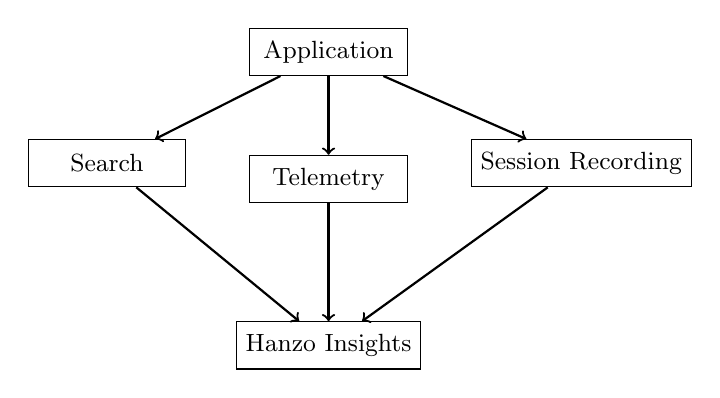
\begin{tikzpicture}[
    node distance=1cm,
    box/.style={rectangle, draw, minimum width=2cm, minimum height=0.6cm, font=\small},
    arrow/.style={->, thick}
]
\node[box] (app) {Application};
\node[box, below left=0.8cm and 0.8cm of app] (search) {Search};
\node[box, below=of app] (telemetry) {Telemetry};
\node[box, below right=0.8cm and 0.8cm of app] (rrweb) {Session Recording};
\node[box, below=1.5cm of telemetry] (insights) {Hanzo Insights};

\draw[arrow] (app) -- (search);
\draw[arrow] (app) -- (telemetry);
\draw[arrow] (app) -- (rrweb);
\draw[arrow] (search) -- (insights);
\draw[arrow] (telemetry) -- (insights);
\draw[arrow] (rrweb) -- (insights);
\end{tikzpicture}
\caption{Observability data flow into Hanzo Insights.}
\end{figure}

All three data streams (search queries, metrics, session recordings) converge in the Hanzo Insights dashboard. Operators can correlate a performance anomaly (telemetry) with the user experience (session recording) and the search queries that led to the affected page.

\section{Operational Scale}

\begin{table}[h]
\centering
\caption{Observability stack operational metrics (2018).}
\begin{tabular}{lr}
\toprule
\textbf{Metric} & \textbf{Value} \\
\midrule
Search index size & 2.4 TB \\
Queries per second (search) & 12{,}000 \\
Metrics time series (active) & 1{,}200{,}000 \\
Scrape interval & 15 s \\
Session recordings per day & 85{,}000 \\
Mean recording size & 340 KB \\
Event ingestion rate & 45{,}000 events/s \\
\bottomrule
\end{tabular}
\end{table}

\section{Conclusion}

The Hanzo observability stack provides full-text search, metrics collection, session recording, and event analytics as a unified platform. The system evolved from an OpenAPI specification layer (2016) into a comprehensive observability solution by late 2018. Privacy-first design, multi-tenant isolation, and integration with the Hanzo PubSub event bus ensure that observability data is collected, stored, and queried without exposing sensitive user information across tenant boundaries. This infrastructure became the foundation for Hanzo Insights, the analytics product offered to Hanzo platform tenants.

\bibliographystyle{plain}
\begin{thebibliography}{9}

\bibitem{bm25}
S.~Robertson and H.~Zaragoza. The probabilistic relevance framework: BM25 and beyond. \textit{Foundations and Trends in Information Retrieval}, 3(4):333--389, 2009.

\bibitem{prometheus2015}
Prometheus Authors. Prometheus: Monitoring system and time series database. \url{https://prometheus.io}, 2015.

\bibitem{rrweb2018}
Y.~Yin. rrweb: Record and replay the web. \url{https://rrweb.io}, 2018.

\bibitem{openapi2016}
OpenAPI Initiative. OpenAPI Specification 3.0. \url{https://openapis.org}, 2016.

\end{thebibliography}

\end{document}
